%%%%%%%%%%MODULI
\section{Organizzazione dei componenti, i Moduli}
Uno dei concetti principali del framework Angular è il rendere le applicazioni il più modulari possibile. Per realizzarla la libreria propone il concetto di ngModule, un ngModule consiste in un raggruppamento di entità angular dedicate all'implementazione di una particolare sotto funzionalità, un servizio necessario all'applicazione o un particolare step dell'applicazione.
Un ngModule può contenere al suo interno:
\begin{itemize}
    \item Componenti
    \item Service
    \item Qualunque altro file utile allo sviluppo della funzionalità offerta dal modulo
\end{itemize}
Ogni applicazione Angular è formata da un insieme di ngModule dei quali ne è sempre presente uno radice (root) il quale viene lanciato all'avvio dell'applicazione.
Cosi come i componenti, anche gli ngModule sono organizzati in una struttura ad albero,
della quale la radice è l' ngModule root 
\subsection{Metadati}
un ngModule è definito da una classe typescript con decorator @ngModule il quale definisce i suoi metadati:
\begin{itemize}
    \item La lista di componenti direttive e service che fanno parte del ngModule
    \item Gli elementi che sono visibili e utilizzabili dagli altri moduli
    \item Gli elementi che sono importati da altri moduli
    \item Tutti i fornitori di service che questo modulo espone all'esterno
    \item Il componente root del modulo
\end{itemize}
Ogni ngModule crea un ambiente di compilazione isolato per le entità al suo interno e possiede un componente root che viene caricato al boot, ma è comunque possibile accedere agli altri componenti del ngModule tramite il routing o il rendering del template del singolo componente
\begin{figure}[H]
    \centering
   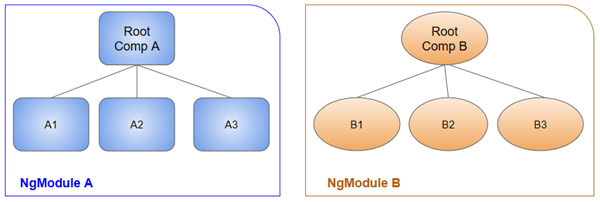
\includegraphics[scale=1]{resources/compilation-context.png}
   \cite{angular-doc}
    \caption{rappresentazione ambiente di compilazione dei moduli}
\end{figure}


come mostrato nell'immagine i due ngModule offrono ambienti di compilazione differenti per i moduli all'interno, questo consente alle applicazioni angular di essere pienamente modulari dato che i singoli moduli sono pienamente indipendenti.
\newline
Come mostrato dall'immagine sottostante, le view possono essere organizzate in gerarchie, che rappresentano singole aree di visualizzazione all'interno della pagina,esse vengono gestite dalla libreria come una unica entità e possono contenere componenti da ngModule differenti
\begin{figure}[H]
    \centering
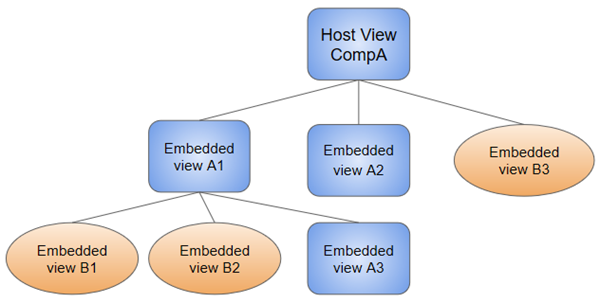
\includegraphics[scale=1]{resources/view-hierarchy.png}
   \cite{angular-doc}
    \caption{rappresentazione gerarchia delle view}
\end{figure}
\newpage
